\documentclass[10pt,a4,]{article}
\usepackage[dvipsnames]{xcolor}
% \RequirePackage[l2tabu, orthodox]{nag}
\usepackage[a4paper,text={16.5cm,25.2cm},centering,margin=2.4cm]{geometry}
% \usepackage[left=1.0in,top=1.0in,right=1.0in,bottom=1.0in]{geometry}
\newcommand*{\authorfont}{\fontfamily{phv}\selectfont}
\usepackage{hyperref,amsmath,amssymb,bm,url,enumitem,dcolumn,upquote,framed,alltt,textgreek,xfrac,fixltx2e}
\usepackage[australian]{babel}
\usepackage[compact,small]{titlesec}
\setlength{\parskip}{1.2ex}
\setlength{\parindent}{0em}

\def\tightlist{}

\usepackage{ifxetex}
\ifxetex
 \usepackage{fontspec}
 \defaultfontfeatures{Ligatures=TeX} % To support LaTeX quoting style
 % \defaultfontfeatures{Ligatures=TeX,Numbers={OldStyle}}
 \setmainfont{Palatino}
 \setsansfont[Scale=MatchLowercase]{Avenir Next Condensed}
 \setmonofont[Scale=0.78,Color=RubineRed]{Bitstream Vera Sans Mono}
\else
  \usepackage[T1]{fontenc}
  \usepackage[utf8]{inputenc}
  \usepackage{lmodern}
  % \usepackage[full]{textcomp} % directly use the degree (and some other) symbol
\fi

% place after fonts; even better typesetting for improved readability:
\graphicspath{ {figure/} }
\usepackage{tabularx} % for 'tabularx' environment and 'X' column type
\usepackage{ragged2e}  % for '\RaggedRight' macro (allows hyphenation)
\usepackage{siunitx}
    \sisetup{%
        detect-mode,
        group-digits            = false,
        input-symbols           = ( ) [ ] - + < > *,
        table-align-text-post   = false,
        round-mode              = places,
        round-precision         = 3
        }
% \usepackage[font={small, sf}, labelfont=bf]{caption} % tweaking the captions
\usepackage[font={small}, labelfont=bf]{caption} % tweaking the captions
\usepackage[color=yellow, textsize=tiny]{todonotes}
\frenchspacing%

\usepackage{abstract}
\renewcommand{\abstractname}{} % clear the title
\renewcommand{\absnamepos}{empty} % originally center

\renewenvironment{abstract}
{{%
\setlength{\leftmargin}{0mm}
\setlength{\rightmargin}{\leftmargin}%
}%
\relax}
{\endlist}

\makeatletter
\def\@maketitle{%
\newpage
%  \null
%  \vskip 2em%
%  \begin{center}%
\let \footnote \thanks
 {\fontsize{18}{20}\selectfont\raggedright  \setlength{\parindent}{0pt} \@title \par}%
}
%\fi
\makeatother


\setcounter{secnumdepth}{0}



\usepackage{color}
\usepackage{fancyvrb}
\newcommand{\VerbBar}{|}
\newcommand{\VERB}{\Verb[commandchars=\\\{\}]}
\DefineVerbatimEnvironment{Highlighting}{Verbatim}{commandchars=\\\{\}}
% Add ',fontsize=\small' for more characters per line
\usepackage{framed}
\definecolor{shadecolor}{RGB}{248,248,248}
\newenvironment{Shaded}{\begin{snugshade}}{\end{snugshade}}
\newcommand{\AlertTok}[1]{\textcolor[rgb]{0.94,0.16,0.16}{#1}}
\newcommand{\AnnotationTok}[1]{\textcolor[rgb]{0.56,0.35,0.01}{\textbf{\textit{#1}}}}
\newcommand{\AttributeTok}[1]{\textcolor[rgb]{0.77,0.63,0.00}{#1}}
\newcommand{\BaseNTok}[1]{\textcolor[rgb]{0.00,0.00,0.81}{#1}}
\newcommand{\BuiltInTok}[1]{#1}
\newcommand{\CharTok}[1]{\textcolor[rgb]{0.31,0.60,0.02}{#1}}
\newcommand{\CommentTok}[1]{\textcolor[rgb]{0.56,0.35,0.01}{\textit{#1}}}
\newcommand{\CommentVarTok}[1]{\textcolor[rgb]{0.56,0.35,0.01}{\textbf{\textit{#1}}}}
\newcommand{\ConstantTok}[1]{\textcolor[rgb]{0.00,0.00,0.00}{#1}}
\newcommand{\ControlFlowTok}[1]{\textcolor[rgb]{0.13,0.29,0.53}{\textbf{#1}}}
\newcommand{\DataTypeTok}[1]{\textcolor[rgb]{0.13,0.29,0.53}{#1}}
\newcommand{\DecValTok}[1]{\textcolor[rgb]{0.00,0.00,0.81}{#1}}
\newcommand{\DocumentationTok}[1]{\textcolor[rgb]{0.56,0.35,0.01}{\textbf{\textit{#1}}}}
\newcommand{\ErrorTok}[1]{\textcolor[rgb]{0.64,0.00,0.00}{\textbf{#1}}}
\newcommand{\ExtensionTok}[1]{#1}
\newcommand{\FloatTok}[1]{\textcolor[rgb]{0.00,0.00,0.81}{#1}}
\newcommand{\FunctionTok}[1]{\textcolor[rgb]{0.00,0.00,0.00}{#1}}
\newcommand{\ImportTok}[1]{#1}
\newcommand{\InformationTok}[1]{\textcolor[rgb]{0.56,0.35,0.01}{\textbf{\textit{#1}}}}
\newcommand{\KeywordTok}[1]{\textcolor[rgb]{0.13,0.29,0.53}{\textbf{#1}}}
\newcommand{\NormalTok}[1]{#1}
\newcommand{\OperatorTok}[1]{\textcolor[rgb]{0.81,0.36,0.00}{\textbf{#1}}}
\newcommand{\OtherTok}[1]{\textcolor[rgb]{0.56,0.35,0.01}{#1}}
\newcommand{\PreprocessorTok}[1]{\textcolor[rgb]{0.56,0.35,0.01}{\textit{#1}}}
\newcommand{\RegionMarkerTok}[1]{#1}
\newcommand{\SpecialCharTok}[1]{\textcolor[rgb]{0.00,0.00,0.00}{#1}}
\newcommand{\SpecialStringTok}[1]{\textcolor[rgb]{0.31,0.60,0.02}{#1}}
\newcommand{\StringTok}[1]{\textcolor[rgb]{0.31,0.60,0.02}{#1}}
\newcommand{\VariableTok}[1]{\textcolor[rgb]{0.00,0.00,0.00}{#1}}
\newcommand{\VerbatimStringTok}[1]{\textcolor[rgb]{0.31,0.60,0.02}{#1}}
\newcommand{\WarningTok}[1]{\textcolor[rgb]{0.56,0.35,0.01}{\textbf{\textit{#1}}}}


\usepackage{longtable,booktabs}
\setlength\heavyrulewidth{0.1em}
\setlength\lightrulewidth{0.0625em}


\title{The Seaweeds in Two Oceans Data  }

\author{\Large AJ
Smit\vspace{0.05in} \newline\normalsize\emph{University of the Western
Cape}  }

\date{}

% PENALTIES
\widowpenalty=1000
\clubpenalty=1000
\doublehyphendemerits=9999 % Almost no consecutive line hyphens
\brokenpenalty=10000 % No broken words across columns/pages
\interfootnotelinepenalty=9999 % Almost never break footnotes

% SECTION, SUBSECETC.TITLES
\usepackage[compact]{titlesec}
\titleformat{\chapter}
  {\normalfont\LARGE\sffamily\bfseries}
  {\thechapter}
  {1em}
  {}
\titleformat{\section}
  {\normalfont\LARGE\sffamily\bfseries}
  {\thesection}
  {1em}
  {}
\titleformat{\subsection}
  {\normalfont\Large\sffamily\bfseries}
  {\thesubsection}
  {1em}
  {}
\titleformat{\subsubsection}
  {\normalfont\large\sffamily\bfseries\slshape}
  {\thesubsubsection}
  {1em}
  {}
% \titlespacing*{<command>}{<left>}{<before-sep>}{<after-sep>}
\titlespacing*{\chapter}
  {0pt}
  {1.2ex plus 1ex minus .2ex}
  {0.5ex plus .1ex minus .1ex}
\titlespacing*{\section}
  {0pt}
  {1.2ex plus 1ex minus .2ex}
  {0.5ex plus .1ex minus .1ex}
\titlespacing*{\subsection}
  {0pt}
  {1.2ex plus 1ex minus .2ex}
  {0.5ex plus .1ex minus .1ex}
\titlespacing*{\subsubsection}
  {0pt}
  {1.2ex plus 1ex minus .2ex}
  {0.5ex plus .1ex minus .1ex}

\newlength{\cslhangindent}
\setlength{\cslhangindent}{1.5em}
\newenvironment{cslreferences}%
  {\setlength{\parindent}{0pt}%
  \everypar{\setlength{\hangindent}{\cslhangindent}}\ignorespaces}%
  {\par}



\newtheorem{hypothesis}{Hypothesis}
\usepackage{setspace}

\makeatletter

\@ifpackageloaded{hyperref}{}{%
\ifxetex
  \usepackage[setpagesize=false, % page size defined by xetex
              unicode=false, % unicode breaks when used with xetex
              xetex]{hyperref}
\else
  \usepackage[colorlinks=true, citecolor=blue, linkcolor=cyan, pdfborder={0 0 0 }, unicode=true]{hyperref} % place after other packages, but before cleveref
\fi
}

\@ifpackageloaded{color}{
    \PassOptionsToPackage{usenames,dvipsnames}{color}
}{%
    \usepackage[usenames,dvipsnames]{color}
}

\usepackage{cleveref} % cleverly cross referencing figures and tables; last package to include
\setcounter{secnumdepth}{2}
\setcounter{tocdepth}{2}

% To use for resetting the numbering of Appendix Tables and Figures:
%\setcounter{table}{0}
%\renewcommand{\thetable}{A\arabic{table}}
%\setcounter{figure}{0}
%\renewcommand{\thefigure}{A\arabic{figure}}

\makeatother
\hypersetup{breaklinks=true,
            bookmarks=true,
            pdfauthor={AJ Smit (University of the Western Cape)},
             pdfkeywords = {},
            pdftitle={The Seaweeds in Two Oceans Data},
            colorlinks=true,
            citecolor=blue,
            urlcolor=blue,
            linkcolor=magenta,
            pdfborder={0 0 0}}
\urlstyle{same}  % don't use monospace font for urls


\begin{document}

% \maketitle

{% \usefont{T1}{pnc}{m}{n}
\setlength{\parindent}{0pt}
\thispagestyle{plain}
{\fontsize{18}{20}\selectfont\raggedright
\maketitle  % title \par
}
{
   \vskip 13.5pt\relax \normalsize\fontsize{11}{12}
\textbf{\authorfont AJ Smit} \hskip 15pt \emph{\small University of the
Western Cape}   
}
}



\vskip 6.5pt

\noindent 

\section{The South African seaweed data}

The data were collected for the regions defined in the table, below:

\begin{tiny}
\begin{center}
\setlength\tabcolsep{4pt}
\begin{longtable}{|r|r|r|l|p{6cm}|}
\caption{The 58 \texttimes{} 50 km sections of the South African coastline, with approximate GPS coordinates, delineation of sections, and some well-known sites in each section. Taken with permission from Bolton and Stegenga (2002).} \\

% This is the header for the first page of the table...
\toprule
Site & Lon & Lat & Limits & Including \\
\midrule
\endfirsthead

% This is the header for the second page of the table...
\toprule
Site & Lon & Lat & Limits & Including \\
\midrule
\endhead

% This is the footer for all pages except the last page of the table...
\midrule
\multicolumn{5}{l}{{Continued on Next Page\ldots}} \\
\endfoot

% This is the footer for the last page of the table...
\bottomrule
\endlastfoot

% Now the data...
1 & 16.72 & -28.98 & Orange River to just south of Holgats River  &  \\
2 & 16.94 & -29.38 & To just south of Wedge Point & Port Nolloth \\
3 & 17.08 & -29.83 & To just south of Melkbos Point & Kleinzee \\
4 & 17.26 & -30.26 & To Swartlintjies River & Skulpfontein Point, Swartlintjies \\
5 & 17.48 & -30.68 & To 10 km north of Groen River  & River Hondeklip Bay, Spoeg River \\
6 & 17.72 & -31.09 & To just north of Brak River & Groen River, Island Point, Blougat \\
7 & 18.00 & -31.46 & To just north of Duiwegat & Voëlklip, Sout River, Blinkwater Bay \\
8 & 18.25 & -31.85 & To just south of Doring Bay & Olifants River, Strandfontein, Doring Bay \\
9 & 18.34 & -32.30 & To just north of Elands Bay & Lambert’s Bay, Lang River \\
10 & 18.20 & -32.72 & To just north of Laaiplek & Elands Bay, Die Vlei, Dwarskersbos \\
11 & 17.85 & -32.83 & To just south of Cape Columbine & Laaiplek, St Helena Bay, Paternoster \\
12 & 18.03 & -33.03 & To just east of Saldahna &  \\
13 & 18.01 & -33.15 & To Postberg & Langebaan Lagoon \\
14 & 18.32 & -33.50 & To just south of Modder River & Yzerfontein, Dassen Is., Grotto Bay \\
15 & 18.47 & -33.91 & To Sea Point & Melkbosstrand, Table Bay, Green Point \\
16 & 18.37 & -34.21 & To just north of Scarborough & Camps Bay, Hout Bay, Kommetjie \\
17 & 18.47 & -34.11 & To just east of Kalk Bay & Scarborough, Cape Point, Fishoek \\
18 & 18.82 & -34.19 & To just south of Gordons Bay & Muizenburg, Strandfontein, Strand \\
19 & 19.07 & -34.35 & To just east of Kleinmond & Rooi Els, Hangklip, Betty’s Bay \\
20 & 19.34 & -34.59 & To just south of Danger Point & Bot River, Sand Bay, Hermanus, Die Kelders \\
21 & 19.66 & -34.79 & To just east of Quoin Point & Danger Point, Pearly Beach, Dyer Island \\
22 & 20.07 & -34.75 & To just east of Struis Bay & Die Mond, Cape Agulhas \\
23 & 20.48 & -34.49 & To just east of Skipskop & Struis Bay, Arniston \\
24 & 20.87 & -34.39 & To just east of Cape Infanta & Koppie Alleen, Cape Infanta, Bree River, Witsand \\
25 & 21.36 & -34.42 & To just east of Grootjongensfontein & Puntjie, Skurwe Bay \\
26 & 21.83 & -34.38 & To just west of Gouritzmond & Stil Bay, Bloukrans, Bull Point \\
27 & 22.12 & -34.16 & To just north of Mossel Bay & Gouritzmond, Vlees Bay, Pinnacle Rock \\
28 & 22.54 & -34.01 & To just west of Victoria Bay & Hartenbos, Klein and Groot Brak rivers, Herolds Bay, Skuinsbank \\
29 & 23.02 & -34.08 & To just west of The Heads, Knysna & Victoria Bay, Wilderness, Platbank, Oesterbank, Walker Bay \\
30 & 23.36 & -34.10 & To Jack’s Point, south of Plettenberg Bay  & The Heads, Neusgate \\
31 & 23.78 & -34.01 & To Elandbos River & Plettenberg Bay, Arch Rock, Die Punt, Blousloep \\
32 & 24.27 & -34.08 & To Skuinsklip & Storms River, Voëlkrans, Skietgate \\
33 & 24.74 & -34.19 & To Thys Point & Aasvoëlklip, Tsitsikamma River, Klipdrif River \\
34 & 25.04 & -33.97 & To just west of Gamtoos River & Cape St Francis, Krom River, Seekoei River, Jeffreys Bay \\
35 & 25.52 & -34.04 & To just east of Sardinia Bay & Van Stadens River, Claasen Point \\
36 & 25.70 & -33.79 & To just east of St George’s Beach & Chelsea Point, Port Elizabeth, Bluewater Bay \\
37 & 26.18 & -33.72 & To just west of Woody Cape & St Croix Is., Sundays River \\
38 & 26.65 & -33.70 & To just west of Kenton-on-Sea & Seal Is., Bird Is., Cape Padrone, Cannon Rocks, Boknes \\
39 & 27.10 & -33.52 & To just east of Kleinemonde & Kasouga, Port Alfred \\
40 & 27.52 & -33.27 & To just east of Keiskamma River & Great Fish River, Madagascar Reef \\
41 & 27.93 & -33.01 & To just east of East London & Kayser’s Beach, Kidd’s Beach, Cove Rock \\
42 & 28.30 & -32.73 & To Haga-Haga & Gonubie, Cintsa River \\
43 & 28.68 & -32.44 & To Qora River & Morgans Bay, Kei Mouth, Nxaxo River, Mazeppa Bay \\
44 & 29.05 & -32.11 & To just east of Xora River & Dwesa, The Haven \\
45 & 29.37 & -31.76 & To Sharks Point & Mncwasa River, Coffee Bay, Hluleka \\
46 & 29.74 & -31.46 & To Mkozi River & Boulder Bay, Port St Johns, Montshe, Ntsubane \\
47 & 30.12 & -31.18 & To Mnyameni River & Cathedral Rock, Lambasi Bay, Wild Coast \\
48 & 30.41 & -30.81 & To just north of St Michaels-on-Sea & Mzamba, Port Edward, Southbroom, Margate \\
49 & 30.68 & -30.41 & To just south of Pennington & Port Shepstone, Mzumbe, Sezela \\
50 & 30.93 & -30.01 & To just south of Isipingo Beach & Scottburgh, Park Rynie, Umkomaas, Illovo, Amanzimtoti \\
51 & 31.15 & -29.62 & To Desainagar & Durban, Umhlanga Rocks, Umdloti Beach \\
52 & 31.46 & -29.26 & To just north of Zinkwazi Beach & Westbrook, Ballito, Blythdale Beach \\
53 & 31.82 & -28.94 & To just east of Mtunzini & Tugela River, Dunn’s Reserve \\
54 & 32.21 & -28.70 & To Mbonambi Beach & Richards Bay \\
55 & 32.46 & -28.32 & To just north of First Rocks & Dawson’s Rocks, Cape St Lucia, St Lucia \\
56 & 32.59 & -27.87 & To Bhukwini & Mission Rocks, Cape Vidal, Leven Point \\
57 & 32.72 & -27.42 & To just north of Gobey’s Point & Liefeldts Rocks, Sodwana Bay \\
58 & 32.87 & -26.97 & To Kosimeer & Hulley Point, Black Rock \\

\end{longtable}
\end{center}
\end{tiny}

I use two data sets. The first, \(Y\) (in the file `seaweeds.csv')
comprises distribution records of 847 macroalgal species within each of
58 × 50 km-long sections of the South African coast (updated from Bolton
and Stegenga, 2002). This represents \emph{ca}. 90\% of the known
seaweed flora of South Africa, but excludes some very small and/or very
rare species for which data are insufficient. The data are from
verifiable literature sources and John Bolton and Rob Anderson's own
collections, assembled from information collected by teams of
phycologists over three decades (Bolton, 1986; Bolton and Stegenga,
2002; De Clerck et al., 2005; Stegenga et al., 1997). The second, \(E\)
(in `env.csv'), is a dataset of \emph{in situ} coastal seawater
temperatures (Smit et al., 2013) derived from daily measurements over up
to 40 years.

\section{Setting up the analysis environment}

This is \textbf{R}, so first I need to find, install and load various
packages. Some of the packages will be available on CRAN and can be
accessed and installed in the usual way, but others will have to be
downloaded from \href{https://r-forge.r-project.org/R/?group_id=195}{R
Forge}.

\begin{Shaded}
\begin{Highlighting}[]
\KeywordTok{library}\NormalTok{(tidyverse)}
\KeywordTok{library}\NormalTok{(betapart)}
\KeywordTok{library}\NormalTok{(vegan)}
\KeywordTok{library}\NormalTok{(gridExtra)}
\KeywordTok{library}\NormalTok{(BiodiversityR)}
\KeywordTok{library}\NormalTok{(grid)}
\KeywordTok{library}\NormalTok{(gridBase)}
\KeywordTok{library}\NormalTok{(tidyr)}
\end{Highlighting}
\end{Shaded}

\section{Species diversity}

Let's load the data and see how it is structured:

\begin{Shaded}
\begin{Highlighting}[]
\CommentTok{\# Read in the species data:}
\NormalTok{spp <{-}}\StringTok{ }\KeywordTok{read.csv}\NormalTok{(}\StringTok{\textquotesingle{}../exercises/diversity/seaweeds.csv\textquotesingle{}}\NormalTok{)}
\NormalTok{spp <{-}}\StringTok{ }\NormalTok{dplyr}\OperatorTok{::}\KeywordTok{select}\NormalTok{(spp, }\DecValTok{{-}1}\NormalTok{)}

\CommentTok{\# Lets look at the data:}
\KeywordTok{dim}\NormalTok{(spp)}
\end{Highlighting}
\end{Shaded}

\begin{verbatim}
## [1]  58 847
\end{verbatim}

We see that our dataset has 58 rows and 847 columns. What is in the
columns and rows? Start with the first 5 rows and 5 columns:

\begin{Shaded}
\begin{Highlighting}[]
\NormalTok{spp[}\DecValTok{1}\OperatorTok{:}\DecValTok{5}\NormalTok{, }\DecValTok{1}\OperatorTok{:}\DecValTok{5}\NormalTok{]}
\end{Highlighting}
\end{Shaded}

\begin{verbatim}
##   ACECAL ACEMOE ACRVIR AROSP1 ANAWRI
## 1      0      0      0      0      0
## 2      0      0      0      0      0
## 3      0      0      0      0      0
## 4      0      0      0      0      0
## 5      0      0      0      0      0
\end{verbatim}

Now the last 5 rows and 5 columns:

\begin{Shaded}
\begin{Highlighting}[]
\NormalTok{spp[(}\KeywordTok{nrow}\NormalTok{(spp) }\OperatorTok{{-}}\StringTok{ }\DecValTok{5}\NormalTok{)}\OperatorTok{:}\KeywordTok{nrow}\NormalTok{(spp), (}\KeywordTok{ncol}\NormalTok{(spp) }\OperatorTok{{-}}\StringTok{ }\DecValTok{5}\NormalTok{)}\OperatorTok{:}\KeywordTok{ncol}\NormalTok{(spp)]}
\end{Highlighting}
\end{Shaded}

\begin{verbatim}
##    WOMKWA WOMPAC WRAARG WRAPUR WURMIN ZONSEM
## 53      0      0      1      0      0      0
## 54      0      0      1      0      0      0
## 55      0      0      1      0      0      0
## 56      0      1      1      0      1      0
## 57      1      0      1      0      1      0
## 58      0      0      1      0      1      0
\end{verbatim}

So, each of the rows correspond to a site (i.e.~each of the coastal
sections in Table 1), and the columns each contain a species. The
species are arranged alphabetically, and they are indicated by a
six-letter code.

\subsection{Alpha diversity}

We can represent \textalpha-diversity in three ways, i.e.~1) as species
richness (\(S\)), 2) as a univariate diversity index, such as Shannon
diversity (\(H'\)) or Simpson's diversity (\textlambda), or 3) as a
dissimilarity index, e.g.~Bray-Curtis or Jaccard dissimilarities. We
will work through each in turn (but I will cover the dissimilarity
indices under the `Dissimilarity index' section later on).

First, species richness. In the seaweed biodiversity data---because we
view each coastal section as the local scale (the smallest unit of
sampling)---I simply count the number of species within each of the
sections. The \texttt{diversityresult()} function in the
\textbf{BiodiversityR} package does this easily:

\begin{Shaded}
\begin{Highlighting}[]
\NormalTok{spp\_richness <{-}}\StringTok{ }\KeywordTok{diversityresult}\NormalTok{(spp, }\DataTypeTok{index =} \StringTok{\textquotesingle{}richness\textquotesingle{}}\NormalTok{, }\DataTypeTok{method =} \StringTok{\textquotesingle{}each site\textquotesingle{}}\NormalTok{)}
\CommentTok{\# spp\_richness}
\KeywordTok{ggplot}\NormalTok{(}\DataTypeTok{data =}\NormalTok{ spp\_richness, (}\KeywordTok{aes}\NormalTok{(}\DataTypeTok{x =} \DecValTok{1}\OperatorTok{:}\DecValTok{58}\NormalTok{, }\DataTypeTok{y =}\NormalTok{ richness))) }\OperatorTok{+}
\StringTok{  }\KeywordTok{geom\_line}\NormalTok{() }\OperatorTok{+}\StringTok{ }\KeywordTok{xlab}\NormalTok{(}\StringTok{"Coastal section, west to east"}\NormalTok{) }\OperatorTok{+}\StringTok{ }\KeywordTok{ylab}\NormalTok{(}\StringTok{"Species richness"}\NormalTok{)}
\end{Highlighting}
\end{Shaded}

\begin{center}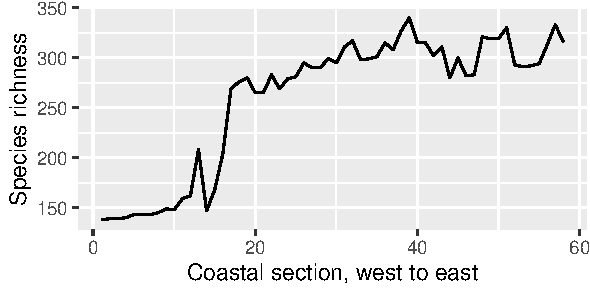
\includegraphics{compliled_figures/unnamed-chunk-3-1} \end{center}

If the \textbf{BiodiversityR} package does not work for you, there is
also the \texttt{specnumber()} function in \textbf{vegan}:

\begin{Shaded}
\begin{Highlighting}[]
\CommentTok{\# Use \textquotesingle{}MARGIN = 1\textquotesingle{} to calculate the number of species within each row (site)}
\KeywordTok{specnumber}\NormalTok{(spp, }\DataTypeTok{MARGIN =} \DecValTok{1}\NormalTok{)}
\end{Highlighting}
\end{Shaded}

\begin{verbatim}
##  [1] 138 139 139 140 143 143 143 145 149 148 159 162 208 147 168 204 269 276 280
## [20] 265 265 283 269 279 281 295 290 290 299 295 311 317 298 299 301 315 308 327
## [39] 340 315 315 302 311 280 300 282 283 321 319 319 330 293 291 292 294 313 333
## [58] 316
\end{verbatim}

In other instances, it makes more sense to calculate the mean species
richness of all the sampling units (e.g.~quadrats) taken inside the
ecosystem of interest. You will have to decide based on your own data.

The second way in which we can express \textalpha-diversity is to use
one of the univariate diversity indices such as Shannon's \(H'\) or
Simpson's \textlambda. Shannon's \(H'\) is sometimes called Shannon's
diversity index, the Shannon--Wiener index, the Shannon--Weaver index,
or the Shannon entropy. It is calculated as

\[\displaystyle H' = -\sum_{i=1}^{R} p_{i} \ln p_{i}\]

where \(p_{i}\) is the proportion of individuals belonging to the
\(i\)th species, and \(R\) is the species richness.

Simpson's \textlambda, or simply the Simpson index, is calculated as

\[\displaystyle \lambda = \sum_{i=1}^{R} p_{i}^{2}\]

where \(R\) is the species richness and \(p_{i}\) is the relative
abundance of the \(i\)th species.

We cannot calculate either of these for the seaweed data because in
order to do so we require abundance data -- the seaweed data are
presence-absence only. Let's load a fictitious dataset of the diversity
of three different communities of plants, with each community
corresponding to a different light environment (dim, mid and high
light):

\begin{Shaded}
\begin{Highlighting}[]
\NormalTok{light <{-}}\StringTok{ }\KeywordTok{read.csv}\NormalTok{(}\StringTok{"../exercises/diversity/light\_levels.csv"}\NormalTok{)}
\NormalTok{light}
\end{Highlighting}
\end{Shaded}

\begin{verbatim}
##         Site    A    B    C    D    E    F
## 1  low_light 0.75 0.62 0.24 0.33 0.21 0.14
## 2  mid_light 0.38 0.15 0.52 0.57 0.28 0.29
## 3 high_light 0.08 0.15 0.18 0.52 0.54 0.56
\end{verbatim}

We can see above that in stead of having data with 1s and 0s for
presence-absence, here we instead have some values that indicate the
relative amounts of each of the species in the three light environments.
We calculate species richness (as before), and also the Shannon and
Simpson indices using \textbf{vegan}'s \texttt{diversity()} function:

\begin{Shaded}
\begin{Highlighting}[]
\NormalTok{light\_div <{-}}\StringTok{ }\KeywordTok{data.frame}\NormalTok{(}
  \DataTypeTok{site =} \KeywordTok{c}\NormalTok{(}\StringTok{"low\_light"}\NormalTok{, }\StringTok{"mid\_light"}\NormalTok{, }\StringTok{"high\_light"}\NormalTok{),}
  \DataTypeTok{richness =} \KeywordTok{specnumber}\NormalTok{(light[, }\DecValTok{2}\OperatorTok{:}\DecValTok{7}\NormalTok{], }\DataTypeTok{MARGIN =} \DecValTok{1}\NormalTok{),}
  \DataTypeTok{shannon =} \KeywordTok{round}\NormalTok{(}\KeywordTok{diversity}\NormalTok{(light[, }\DecValTok{2}\OperatorTok{:}\DecValTok{7}\NormalTok{], }\DataTypeTok{MARGIN =} \DecValTok{1}\NormalTok{, }\DataTypeTok{index =} \StringTok{"shannon"}\NormalTok{), }\DecValTok{2}\NormalTok{),}
  \DataTypeTok{simpson =} \KeywordTok{round}\NormalTok{(}\KeywordTok{diversity}\NormalTok{(light[, }\DecValTok{2}\OperatorTok{:}\DecValTok{7}\NormalTok{], }\DataTypeTok{MARGIN =} \DecValTok{1}\NormalTok{, }\DataTypeTok{index =} \StringTok{"simpson"}\NormalTok{), }\DecValTok{2}\NormalTok{)}
\NormalTok{)}
\NormalTok{light\_div}
\end{Highlighting}
\end{Shaded}

\begin{verbatim}
##         site richness shannon simpson
## 1  low_light        6    1.62    0.78
## 2  mid_light        6    1.71    0.81
## 3 high_light        6    1.59    0.77
\end{verbatim}

\subsection{Gamma diversity}

Returning again to the seaweed data, lets now look at
\textgamma-diversity -- this would simply be the total number of species
along the South African coastline in all 58 coastal sections:

\begin{Shaded}
\begin{Highlighting}[]
\KeywordTok{ncol}\NormalTok{(spp)}
\end{Highlighting}
\end{Shaded}

\begin{verbatim}
## [1] 847
\end{verbatim}

Think before you calculate \textgamma-diversity for your own data as it
might not be as simple as here!

\subsection{Beta diversity}

The first measure of \textbeta-diversity is \emph{true
\textbeta-diversity}. This is simply dividing the \textgamma-diversity
for the region by the \textalpha-diversity for a specific coastal
section. We can calculate it all at once for the whole dataset and make
a graph.

\begin{Shaded}
\begin{Highlighting}[]
\NormalTok{true\_beta <{-}}\StringTok{ }\KeywordTok{data.frame}\NormalTok{(}
  \DataTypeTok{beta =} \KeywordTok{specnumber}\NormalTok{(spp, }\DataTypeTok{MARGIN =} \DecValTok{1}\NormalTok{) }\OperatorTok{/}\StringTok{ }\KeywordTok{ncol}\NormalTok{(spp),}
  \DataTypeTok{section\_no =} \KeywordTok{c}\NormalTok{(}\DecValTok{1}\OperatorTok{:}\DecValTok{58}\NormalTok{)}
\NormalTok{)}
\CommentTok{\# true\_beta}
\KeywordTok{ggplot}\NormalTok{(}\DataTypeTok{data =}\NormalTok{ true\_beta, (}\KeywordTok{aes}\NormalTok{(}\DataTypeTok{x =}\NormalTok{ section\_no, }\DataTypeTok{y =}\NormalTok{ beta))) }\OperatorTok{+}
\StringTok{  }\KeywordTok{geom\_line}\NormalTok{() }\OperatorTok{+}\StringTok{ }\KeywordTok{xlab}\NormalTok{(}\StringTok{"Coastal section, west to east"}\NormalTok{) }\OperatorTok{+}\StringTok{ }\KeywordTok{ylab}\NormalTok{(}\StringTok{"True beta{-}diversity"}\NormalTok{)}
\end{Highlighting}
\end{Shaded}

\begin{center}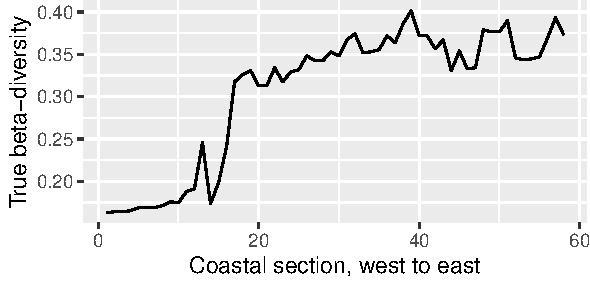
\includegraphics{compliled_figures/unnamed-chunk-8-1} \end{center}

The second measure of \textbeta-diversity is \emph{absolute species
turnover}, and to calculate this we simply simply substract
\textalpha-diversity for each section from the region's
\textgamma-diversity.

\begin{Shaded}
\begin{Highlighting}[]
\NormalTok{abs\_beta <{-}}\StringTok{ }\KeywordTok{data.frame}\NormalTok{(}
  \DataTypeTok{beta =} \KeywordTok{ncol}\NormalTok{(spp) }\OperatorTok{{-}}\StringTok{ }\KeywordTok{specnumber}\NormalTok{(spp, }\DataTypeTok{MARGIN =} \DecValTok{1}\NormalTok{),}
  \DataTypeTok{section\_no =} \KeywordTok{c}\NormalTok{(}\DecValTok{1}\OperatorTok{:}\DecValTok{58}\NormalTok{)}
\NormalTok{)}
\CommentTok{\# abs\_beta}
\KeywordTok{ggplot}\NormalTok{(}\DataTypeTok{data =}\NormalTok{ abs\_beta, (}\KeywordTok{aes}\NormalTok{(}\DataTypeTok{x =}\NormalTok{ section\_no, }\DataTypeTok{y =}\NormalTok{ beta))) }\OperatorTok{+}
\StringTok{  }\KeywordTok{geom\_line}\NormalTok{() }\OperatorTok{+}\StringTok{ }\KeywordTok{xlab}\NormalTok{(}\StringTok{"Coastal section, west to east"}\NormalTok{) }\OperatorTok{+}\StringTok{ }\KeywordTok{ylab}\NormalTok{(}\StringTok{"Absolute beta{-}diversity"}\NormalTok{)}
\end{Highlighting}
\end{Shaded}

\begin{center}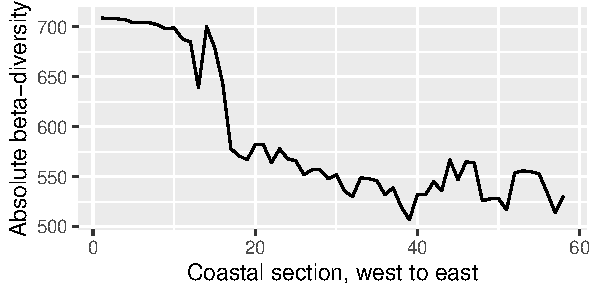
\includegraphics{compliled_figures/unnamed-chunk-9-1} \end{center}

\section{Dissimilarity indices}

In this section we will cover the dissimilarity indices, which are
special cases of diversity indices that use pairwise comparisons between
sampling units, habitats, or ecosystems. Both \textalpha- and
\textbeta-diversity can be expressed as dissimilarity indices, so let us
look at each.

\subsection{Alpha diversity}

Recall from the lecture slides the Bray-Curtis and Jaccard dissimilarity
indices for abundance data, and the Sørensen dissimilarity index for
presence-absence data. The seaweed dataset is a presence-absence
dataset, so we will use the Sørensen index here. The interpretation of
the resulting square dissimilarity matrices is the same regardless of
whether it is calculated from an abundance dataset or a presence-absence
dataset. The values range from 0 to 1, with 0 meaning that the pair of
sites being compared is identical (i.e.~0 dissimilarity) and 1 means the
pair of sites is completely different (no species in common, hence 1
dissimilarity). In the square dissmilarity matrix the diagonal is 0,
which essentially (and obviously) means that any site is identical to
itself. Elsewhere the values will range from 0 to 1. Since this is a
pairwise calculation (each site compared to every other site), our
seaweed dataset will contain (58 × (58 - 1))/2 = 1653 values, each one
ranging from 0 to 1.

The first step involves the species table (\(Y\)). First I compute the
Sørensen dissimilarity index (\(\beta_{\text{sør}}\)) to compare the
dissimilarity of all pairs of coastal sections using on presence-absence
data. The dissimilarity in species composition between two sections is
calculated from three parameters, \emph{viz}., \emph{b} and \emph{c},
which represent the number of species unique to each of two sites, and
\emph{a}, the number of species in common between them. It is given by:

\[\beta_\text{sør}=\frac{b+c}{2a+b+c}\]

\begin{Shaded}
\begin{Highlighting}[]
\NormalTok{sor <{-}}\StringTok{ }\KeywordTok{vegdist}\NormalTok{(spp, }\DataTypeTok{binary =} \OtherTok{TRUE}\NormalTok{)}
\end{Highlighting}
\end{Shaded}

{[}\ldots to be completed\ldots{]}

\subsection{Beta diversity}

β-diversity is a concept that describes how species assemblages
(communities) measured within the ecosystem of interest vary from place
to place, e.g.~between the various transects or quadrats used to sample
the ecosystem. β-diversity results from habitat heterogeneity (along
gradients, or randomly). We have already seen two concepts of
β-diversity, viz.~true β-diversity and absolute species turnover -- both
of these rely on knowledge of species richness at local (a measure of
\textalpha-diversity) and regional (\textgamma-diversity) scales. Much
more insight into species assembly processes can be extracted, however,
when we view \textbeta-diversity as a dissmilarity index. In this view,
we will see that there are two processes by which β-diversity might be
affected (i.e.~in which the patterning of communities over landscapes
might arise):

\begin{description}
\item[Process 1] If a region is comprised of the species A, B, C, …, M (i.e. γ-diversity is 13), a subset of the regional flora as captured by one quadrat might be species \underline{\textbf{A}}, \underline{\textbf{D}}, E, whereas in another quadrat it might be species \underline{\textbf{A}}, \underline{\textbf{D}}, F. In this instance, the α-diversity is 3 in both instances, and heterogeneity (and hence β-diversity) results from the fact that the first quadrat has species E but the other has species F. In other words, here we have the same number of species in both quadrats, but only two of the species are the same. The process responsible for this form of β-diversity is species ‘turnover’ ($\beta_\text{sim}$). Turnover refers to processes that cause communities to differ due to species being lost and/or gained from section to section, i.e. the species composition changes between sections without corresponding changes in α-diversity.

\item[Process 2] Consider again species A, B, C, …, M. Now we have the first quadrat with species \underline{\textbf{A}}, \underline{\textbf{B}}, C, D, \underline{\textbf{G}}, H (α-diversity is 6) and the second quadrat has a subset of this, e.g. only species \underline{\textbf{A}}, \underline{\textbf{B}}, \underline{\textbf{G}} (α-diversity 3). Here, β-diversity comes from the fact that even if the two places share the same species, the number of species can still differ amongst the quadrats (i.e. from place to place) due to one quadrat capturing only a subset of species present in the other. This form of \textbeta-diversity is called ‘nestedness-resultant’ \textbeta-diversity ($\beta_\text{sne}$), and it refers to  processes that cause species to be gained or lost, and the community with the lowest α-diversity is a subset of the richer community.
\end{description}

The above two examples show that β-diversity is coupled not only with
the identity of the species in the quadrats, but also α-diversity --
with species richness in particular.

How do we calculate the turnover and nestedness-resultant components of
\textbeta-diversity? The \textbf{betapart} package (Baselga et al.,
2013) comes to the rescue. I decompose the dissimilarity into the
\(\beta_\text{sim}\) and \(\beta_\text{sne}\) components (Baselga, 2010)
using the \texttt{betapart.core()} and \texttt{betapart.pair()}
functions. The outcomes of this partitioning calculation are placed into
the matrices \(Y1\) and \(Y2\). These data can then be analysed
further---e.g.~I can apply a principal components analysis (PCA) or
another multivariate analysis on \(Y\) to find the major patterns in the
community data--- but I will do this in a later section.

So what can we do with these two forms of \textbeta-diversity? What does
it mean? Let's do a deeper analysis and create a figure to demonstrate
these findings. I regress \(\beta_{\text{sør}}\) on the spatial distance
between section pairs (see below) and on the environmental distance
(\(\beta_{\text{E}}\)) in each bioregion and used the magnitude of the
slope (per 100 km) of this relationship as a metric of beta-diversity or
`distance decay' of dissimilarity. Since the connectivity between
sections is constrained by their location along a shoreline, we
calculated the distances between sections not as `as the crow flies'
distances (e.g.~Section 1 is not connected in a straight line to Section
58 because of the intervening land in-between), but as the great circle
geodesic distances between each pair of sections along a `route'.
Traveling from \textbf{1} to \textbf{58} therefore requires visiting
\textbf{2}, then \textbf{3}, and eventually all the way up to
\textbf{58}. The total distance between a pair of arbitrary sections is
thus the cumulative sum of the great circle distances between each
consecutive pair of intervening sections along the route.

\begin{Shaded}
\begin{Highlighting}[]
\CommentTok{\# Decompose total Sørensen dissimilarity into turnover and nestedness{-}resultant components:}
\NormalTok{Y.core <{-}}\StringTok{ }\KeywordTok{betapart.core}\NormalTok{(spp)}
\NormalTok{Y.pair <{-}}\StringTok{ }\KeywordTok{beta.pair}\NormalTok{(Y.core, }\DataTypeTok{index.family =} \StringTok{"sor"}\NormalTok{)}

\CommentTok{\# Let Y1 be the turnover component (beta{-}sim):}
\NormalTok{Y1 <{-}}\StringTok{ }\KeywordTok{as.matrix}\NormalTok{(Y.pair}\OperatorTok{$}\NormalTok{beta.sim)}
\CommentTok{\# save(Y1, file = "data/Y1.Rdata")}
\CommentTok{\# load("data/Y1.Rdata")}

\CommentTok{\# Let Y2 be the nestedness{-}resultant component (beta{-}sne):}
\NormalTok{Y2 <{-}}\StringTok{ }\KeywordTok{as.matrix}\NormalTok{(Y.pair}\OperatorTok{$}\NormalTok{beta.sne)}
\CommentTok{\# save(Y2, file = "data/Y2.Rdata")}
\CommentTok{\# load("data/Y2.Rdata")}
\end{Highlighting}
\end{Shaded}

\subsection{Principal Components Analysis}

In \textbf{vegan} a PCA is done using the \texttt{rda()} function and
not supplying the constraints (\emph{i.e.} the environment table, \(E\),
or the spatial table, \(S\)). The formal analysis will use the species
data in distance-based redundancy analyses (db-RDA as per
\textbf{vegan}'s \texttt{capscale()} function) by coupling them with
\(E\) and \(S\).

\section{References}

\hypertarget{refs}{}
\begin{cslreferences}
\leavevmode\hypertarget{ref-Baselga2010}{}%
Baselga, A. (2010). Partitioning the turnover and nestedness components
of beta diversity. \emph{Global Ecology and Biogeography} 19, 134--143.

\leavevmode\hypertarget{ref-Baselga2013}{}%
Baselga, A., Orme, D., Villeger, S., Bortoli, J. D., and Leprieur, F.
(2013). \emph{betapart: Partitioning beta diversity into turnover and
nestedness components}. Available at:
\url{http://CRAN.R-project.org/package=betapart}.

\leavevmode\hypertarget{ref-Bolton1986}{}%
Bolton, J. J. (1986). Marine phytogeography of the Benguela upwelling
region on the west coast of southern Africa: A temperature dependent
approach. \emph{Botanica Marina} 29, 251--256.

\leavevmode\hypertarget{ref-Bolton2002}{}%
Bolton, J. J., and Stegenga, H. (2002). Seaweed species diversity in
South Africa. \emph{South African Journal of Marine Science} 24, 9--18.

\leavevmode\hypertarget{ref-DeClerck2005}{}%
De Clerck, O., Bolton, J. J., Anderson, R. J., and Coppejans, E. (2005).
Guide to the seaweeds of KwaZulu-Natal. \emph{Scripta Botanica Belgica}
33, 294 pp.

\leavevmode\hypertarget{ref-Smit2013}{}%
Smit, A. J., Roberts, M., Anderson, R. J., Dufois, F., Dudley, S. F. J.,
Bornman, T. G., et al. (2013). A coastal seawater temperature dataset
for biogeographical studies: large biases between \emph{in situ} and
remotely-sensed data sets around the coast of South Africa. \emph{PLOS
ONE} 8, e81944.

\leavevmode\hypertarget{ref-Stegenga1997}{}%
Stegenga, H., Bolton, J. J., and Anderson, R. J. (1997). Seaweeds of the
South African west coast. \emph{Contributions of the Bolus Herbarium}
18, 3--637.
\end{cslreferences}

\end{document}
